%!TeX root=../tese.tex
%("dica" para o editor de texto: este arquivo é parte de um documento maior)
% para saber mais: https://tex.stackexchange.com/q/78101/183146

\chapter{Dynamic Analysis}
\label{cap:dynamic}

Following the static analysis, we moved on to the dynamic analysis.
Understanding how the recommendation model responds to users reinforcing its
internal biases, like the ones already detected, could potentially lead to a
better understanding of how these systems favor certain kinds of content. We
also were not able to find any published dataset that fit our experimental
design.

The hypothesis is that the recommendation profile will grow even more steep,
which is a reasonable idea; if the users reinforce the beliefs of the algorithm,
then it stands to reason that it will recommend popular items with more and more
frequently, to more and more users. How much more frequently, however, is the
true question.

For the sake of clarity, let us imagine two users with very distinct
preferences: Alice, who enjoys adventure movies, and Bob, who enjoys horror
movies. In principle, the algorithm should have very different recommendations
for both of them and, were they to follow them, their custom suggestions should
grow increasingly different. At the end of this experiment, users like Alice
would all be recommended the same movies, and users like Bob would have their
own set of very popular films; we should expect, therefore, a multimodal
distribution of the recommendation frequencies, with "typical" adventure movies
and "typical" horror movies being much more popular than comedy, for example.

However, if the final recommendation profile looked like what was showcased in
the previous chapter, i.e. a very small subset of movies being recommended to
most users, then we could infer that the system devolved into a degenerate
feedback loop, ignoring personal preferences and distinctions between films.

\section{Datasets}
\label{sec:datasets04}

For the dynamic experiments, we kept using the Movielens dataset
\citep{harper_movielens_2015}. This time, however, we used the full ``1M''
dataset instead of sampling movies from the larger ``25M'' version. Given that
we wanted our dynamic analysis to be conducted in a realistic scenario, we
decided that it would be better not to change the data. This whole experiment
will, therefore, use a version of the dataset commonly used for machine learning
benchmarks with no alteration whatsoever.

The 1M dataset contains 1000209 ratings of almost 4000 movies made by over 6000
anonymous MovieLens users who joined the platform in 2000. In this particular
version, each user has made at least 20 ratings. There are 4 columns available:

\begin{itemize}
  \item \verb|UserID|: Unique user identifier, ranging from 1 to 6040.
  \item \verb|MovieID|: Unique movie identifier, ranging from 1 to 3952.
  \item \verb|Rating|: Movie rating according to user, from 0 to 5 stars.
  \item \verb|Timestamp|: When the user made the rating, in seconds since the
  epoch.
\end{itemize}

A second, auxiliary, dataset was also used to enrich the main one. ``Movies''
contains extra information about the movies in 1M, which allowed us to add more
variables to the recommendation system. This new dataset has 3 columns:

\begin{itemize}
  \item \verb|MovieID|: Unique user identifier, ranging from 1 to 6040.
  \item \verb|Title|: Title of the movie, as provided by IMDB.
  \item \verb|Genres|: Pipe-separated string with all applicable genres.
\end{itemize}

Figure~\ref{fig:fig04_dist_ratings} showcases the distribution of ratings from
the ``1M'' dataset and Figure~\ref{fig:fig04_dist_genres} showcases the
distribution of genres from the ``Movies'' dataset. Note that, for both this
visualization and the rest of the chapter, the genre of each movie is taken to
be the first one listed on the \verb|Genres| column.

\begin{figure}
  \centering
  \begin{subfigure}{0.45\textwidth}
    \centering
    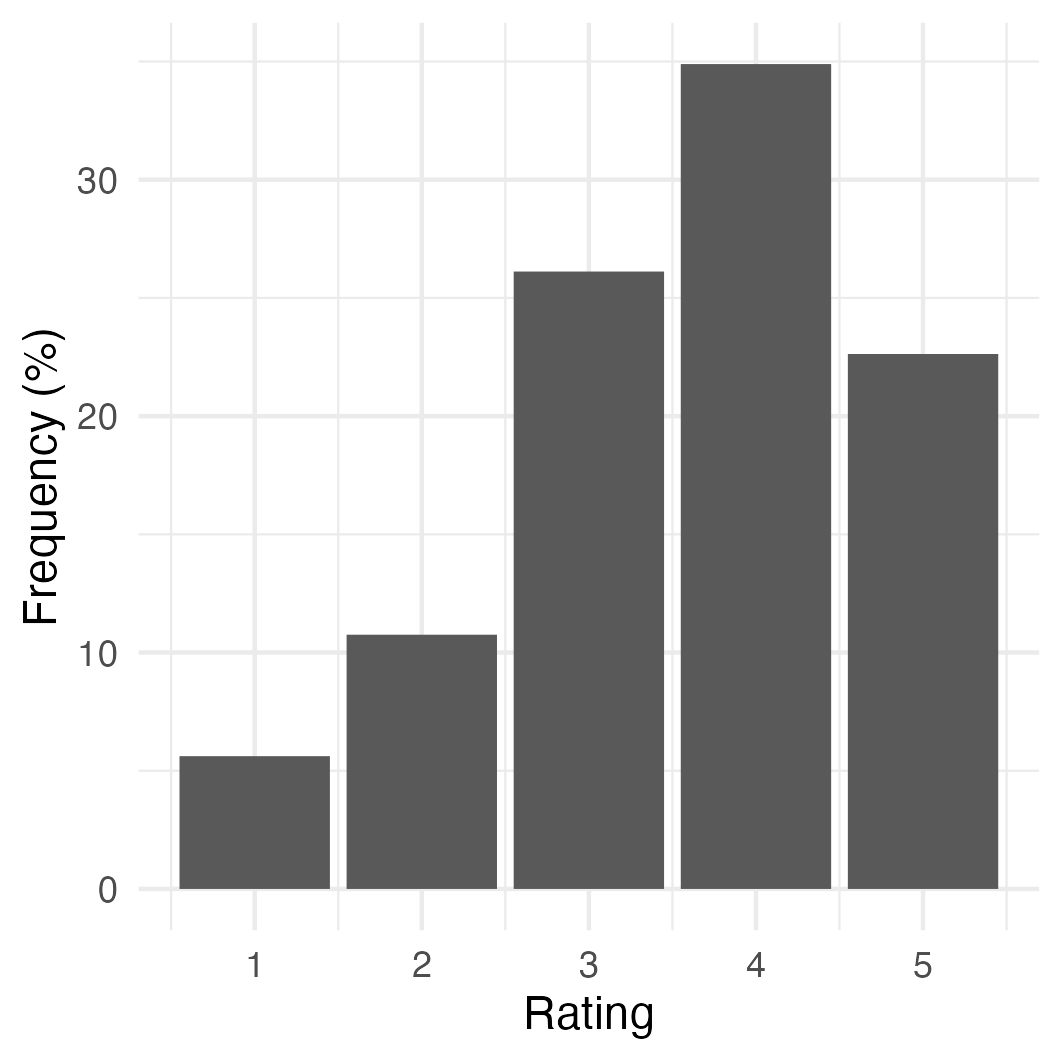
\includegraphics[width=\textwidth]{04_dist_ratings}
    \caption{Rating distribution.\label{fig:fig04_dist_ratings}}
  \end{subfigure}
  \begin{subfigure}{0.45\textwidth}
    \centering
    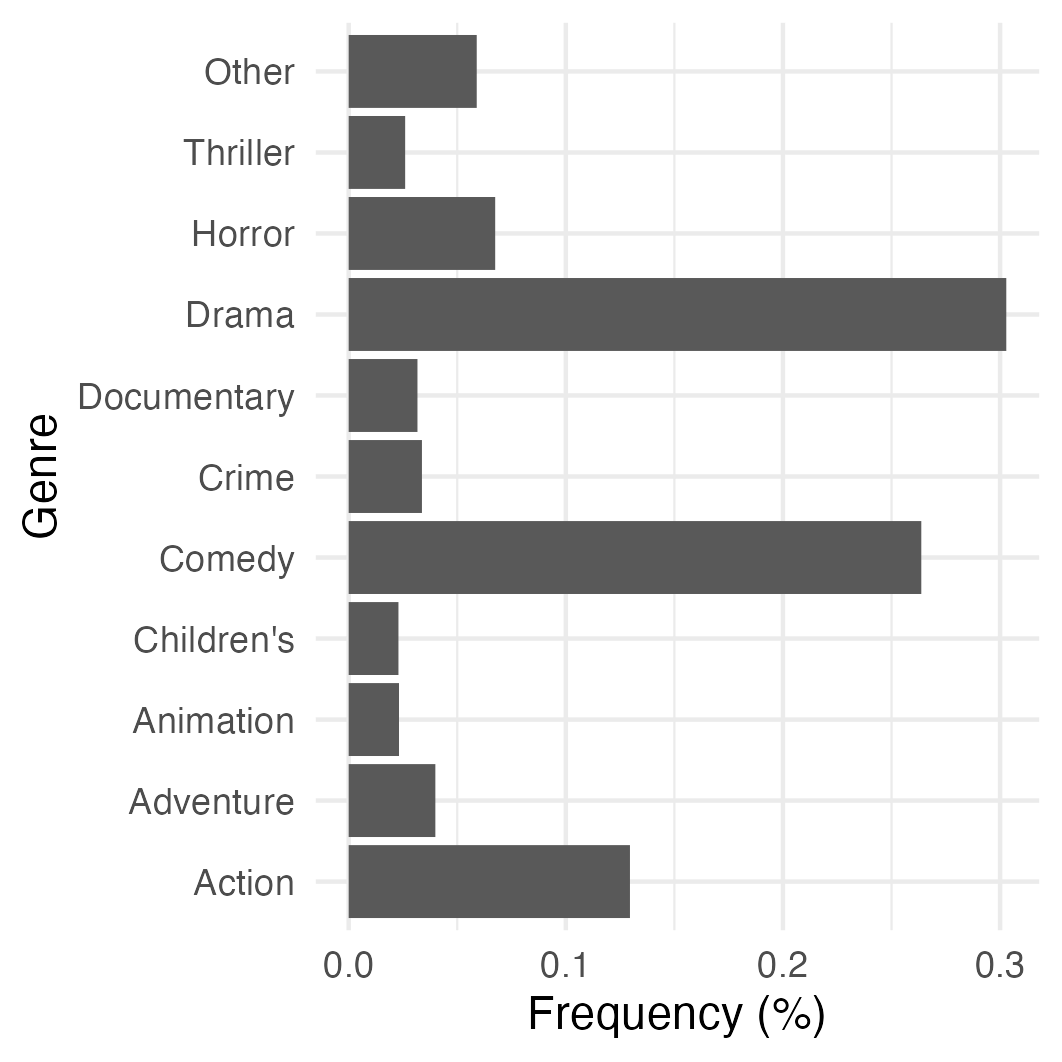
\includegraphics[width=\textwidth]{04_dist_genres}
    \caption{Genre distribution.\label{fig:fig04_dist_genres}}
  \end{subfigure}
  \caption{Distributions of ratings (a) and genres
  (b).\label{fig:fig04_dist_both}}
\end{figure}

\section{Formal Model}

The goal of the dynamic analysis is to better understand how the interaction
between recommendation systems and their users can reinforce internal biases
such as the ones detected in Chapter~\ref{cap:static}.

In order for this analysis to be more robust, we implemented a simple
recommendation algorithm using TensorFlow Recommenders
\citep{noauthor_tensorflow_nodate}, a library for machine learning developed by
Google for use with its TensorFlow \citep{noauthor_tensorflow_nodate-1}
framework. This means that, even though our model is deliberately bare-bones, it
conforms to industry-standard technology and practices.

The choice to use a simple recommendation algorithm instead of a more complex
one was twofold: first, we did not want to use a model that could introduce many
confounding parameters to the analysis (e.g. hyperparameters, hardware
requirements, etc.), and second, we wanted to study a baseline that could, in
the future, be used as a comparison point for more complex algorithms. Our
algorithm is, therefore, a straightforward neural network.

The chosen recommendation algorithm was a basic ranking model described in
\citet{noauthor_recommending_nodate}. It is composed of multiple stacked dense
layers and uses regularized mean squared error as its loss function in order to
avoid overfitting. The main class in the model is reproduced below in
Program~\ref{prog:prog04_tf_model}, and the full algorithm is listed in
Appendix~\ref{apx:model}.

\begin{lstlisting}[language=Python,label=prog:prog04_tf_model,caption=MovielensModel,frame=tb]
class MovielensModel(tfrs.models.Model):

def __init__(self):
  super().__init__()
  self.ranking_model: tf.keras.Model = RankingModel()
  self.task: tf.keras.layers.Layer = tfrs.tasks.Ranking(
    loss = tf.keras.losses.MeanSquaredError(),
    metrics=[tf.keras.metrics.RootMeanSquaredError()]
  )

def call(self, features: Dict[str, tf.Tensor]) -> tf.Tensor:
  return self.ranking_model(
      (features["user_id"], features["movie_title"]))

def compute_loss(self, features: Dict[Text, tf.Tensor],
                  training=False) -> tf.Tensor:
  labels = features.pop("user_rating")

  rating_predictions = self(features)

  # The task computes the loss and the metrics.
  return self.task(labels=labels, predictions=rating_predictions)
\end{lstlisting}

We then trained the recommendation model using Movielens' 1M ratings dataset,
which we will refer to as \verb|ratings0| from now on. Evaluating our model,
called \verb|model0|, on test data yielded a root mean squared error (RMSE) of
0.92; this result is similar to TFRS' deep \& cross network
\citep{wang_deep_2017} results when trained on the same data.

Once \verb|model0| was ready to start making recommendations, we applied it to
every possible user-movie pairing, generating a complete matrix of predicted
ratings called \verb|predictions0|.

A feedback loop, however, cannot be created from a single iteration. In an
environment like YouTube's recommendations sidebar, the user is presented with a
few items that the algorithm thinks they would like, and then they can select
one of the options to watch. We can simulate a user going through this process
by selecting one movie from each user's best-ranked entries in
\verb|predictions0|.

After doing this selection, we can remove the oldest rating of each each user
from \verb|ratings0| and append these these new selections to the dataset in
order to create \verb|ratings1| (a new simulated watch history). The full data
flow is illustrated in Figure~\ref{fig:fig04_dynamic_diagram}.

\begin{figure}
  \centering
  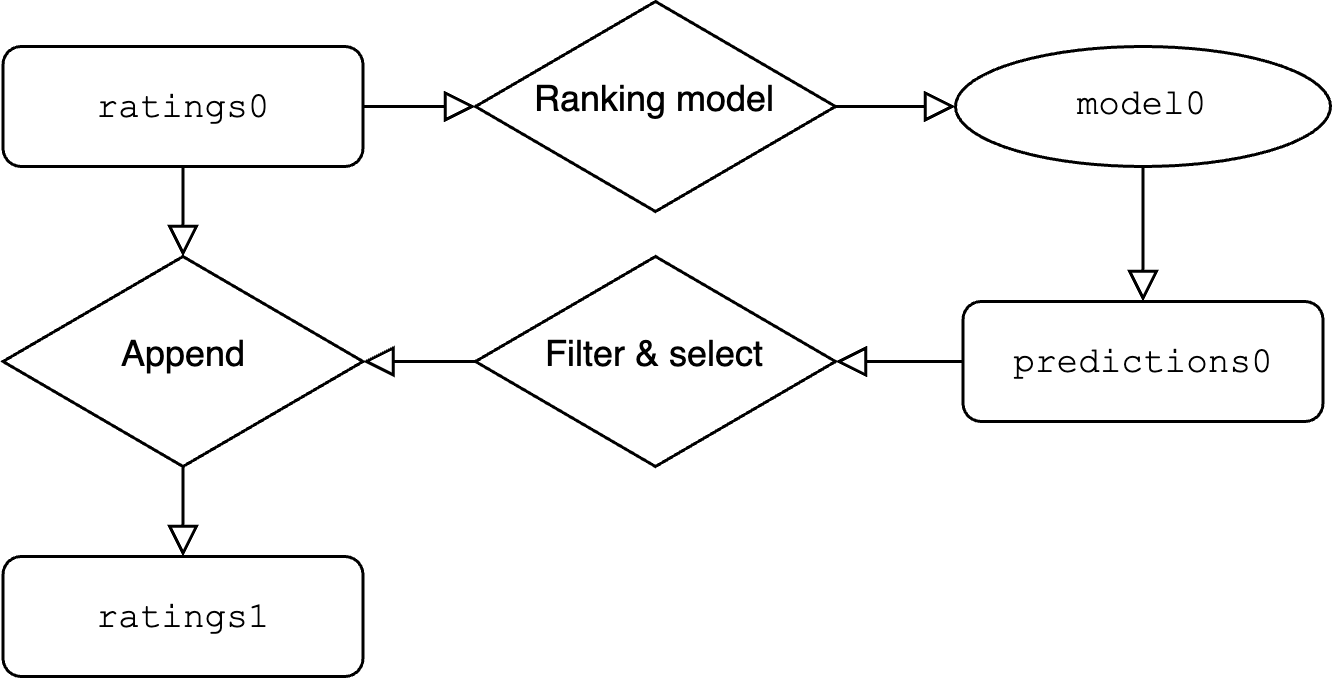
\includegraphics[width=\textwidth]{04_dynamic_diagram}
  \caption{Data flow diagram.\label{fig:fig04_dynamic_diagram}}
\end{figure}

\section{Experiments}
\label{sec:experiments04}

The dynamic experiment starts in a manner much similar to the static experiment.
The full MovieLens dataset is fed as training data to a recommendation system in
order to get it ready for giving suggestions to users. As explained above, we
chose a simple algorithm, (i.e., without rich features or complex layer
arrangements) in order to reduce the number of possible interferences
architecture could have on our analysis.

We repeated the process of creating new watch history datasets and training new
models with them until we got to \verb|ratings4|, totaling 5 ratings datasets
(one original and 4 derived through ranking models). Since we were not taking
personal taste into account, we assumed that no user ever ignores their
recommendations and always picks one movie at random from their own 10
best-ranked recommendations.

With these new datasets we were able to analyze the differences between distinct
generations of models and understand exactly how the positive feedback loop
influenced the last iteration.

Figure~\ref{fig:fig04_profile_grouped} has five subplots which represent the
recommendation profile of each iteration of the recommendation system. For
\verb|ratings0|, it is possible to see that a number of well-rated movies were
more popular, i.e., were rated by more people. Once we generate the first batch
of recommendations, we add up the number of users each movie was recommended to;
this is seen in the second plot, \verb|ratings1|. The outlier points to the left
clearly indicate that a small subset of movies strayed from the pack and were
recommended to more people than had watched them previously.

This process repeats itself until, in \verb|ratings4|, the most popular movie is
recommended more than 2000 times, while the most popular movie in
\verb|ratings0| was watched a little over 500 times.

\begin{figure}
  \centering
  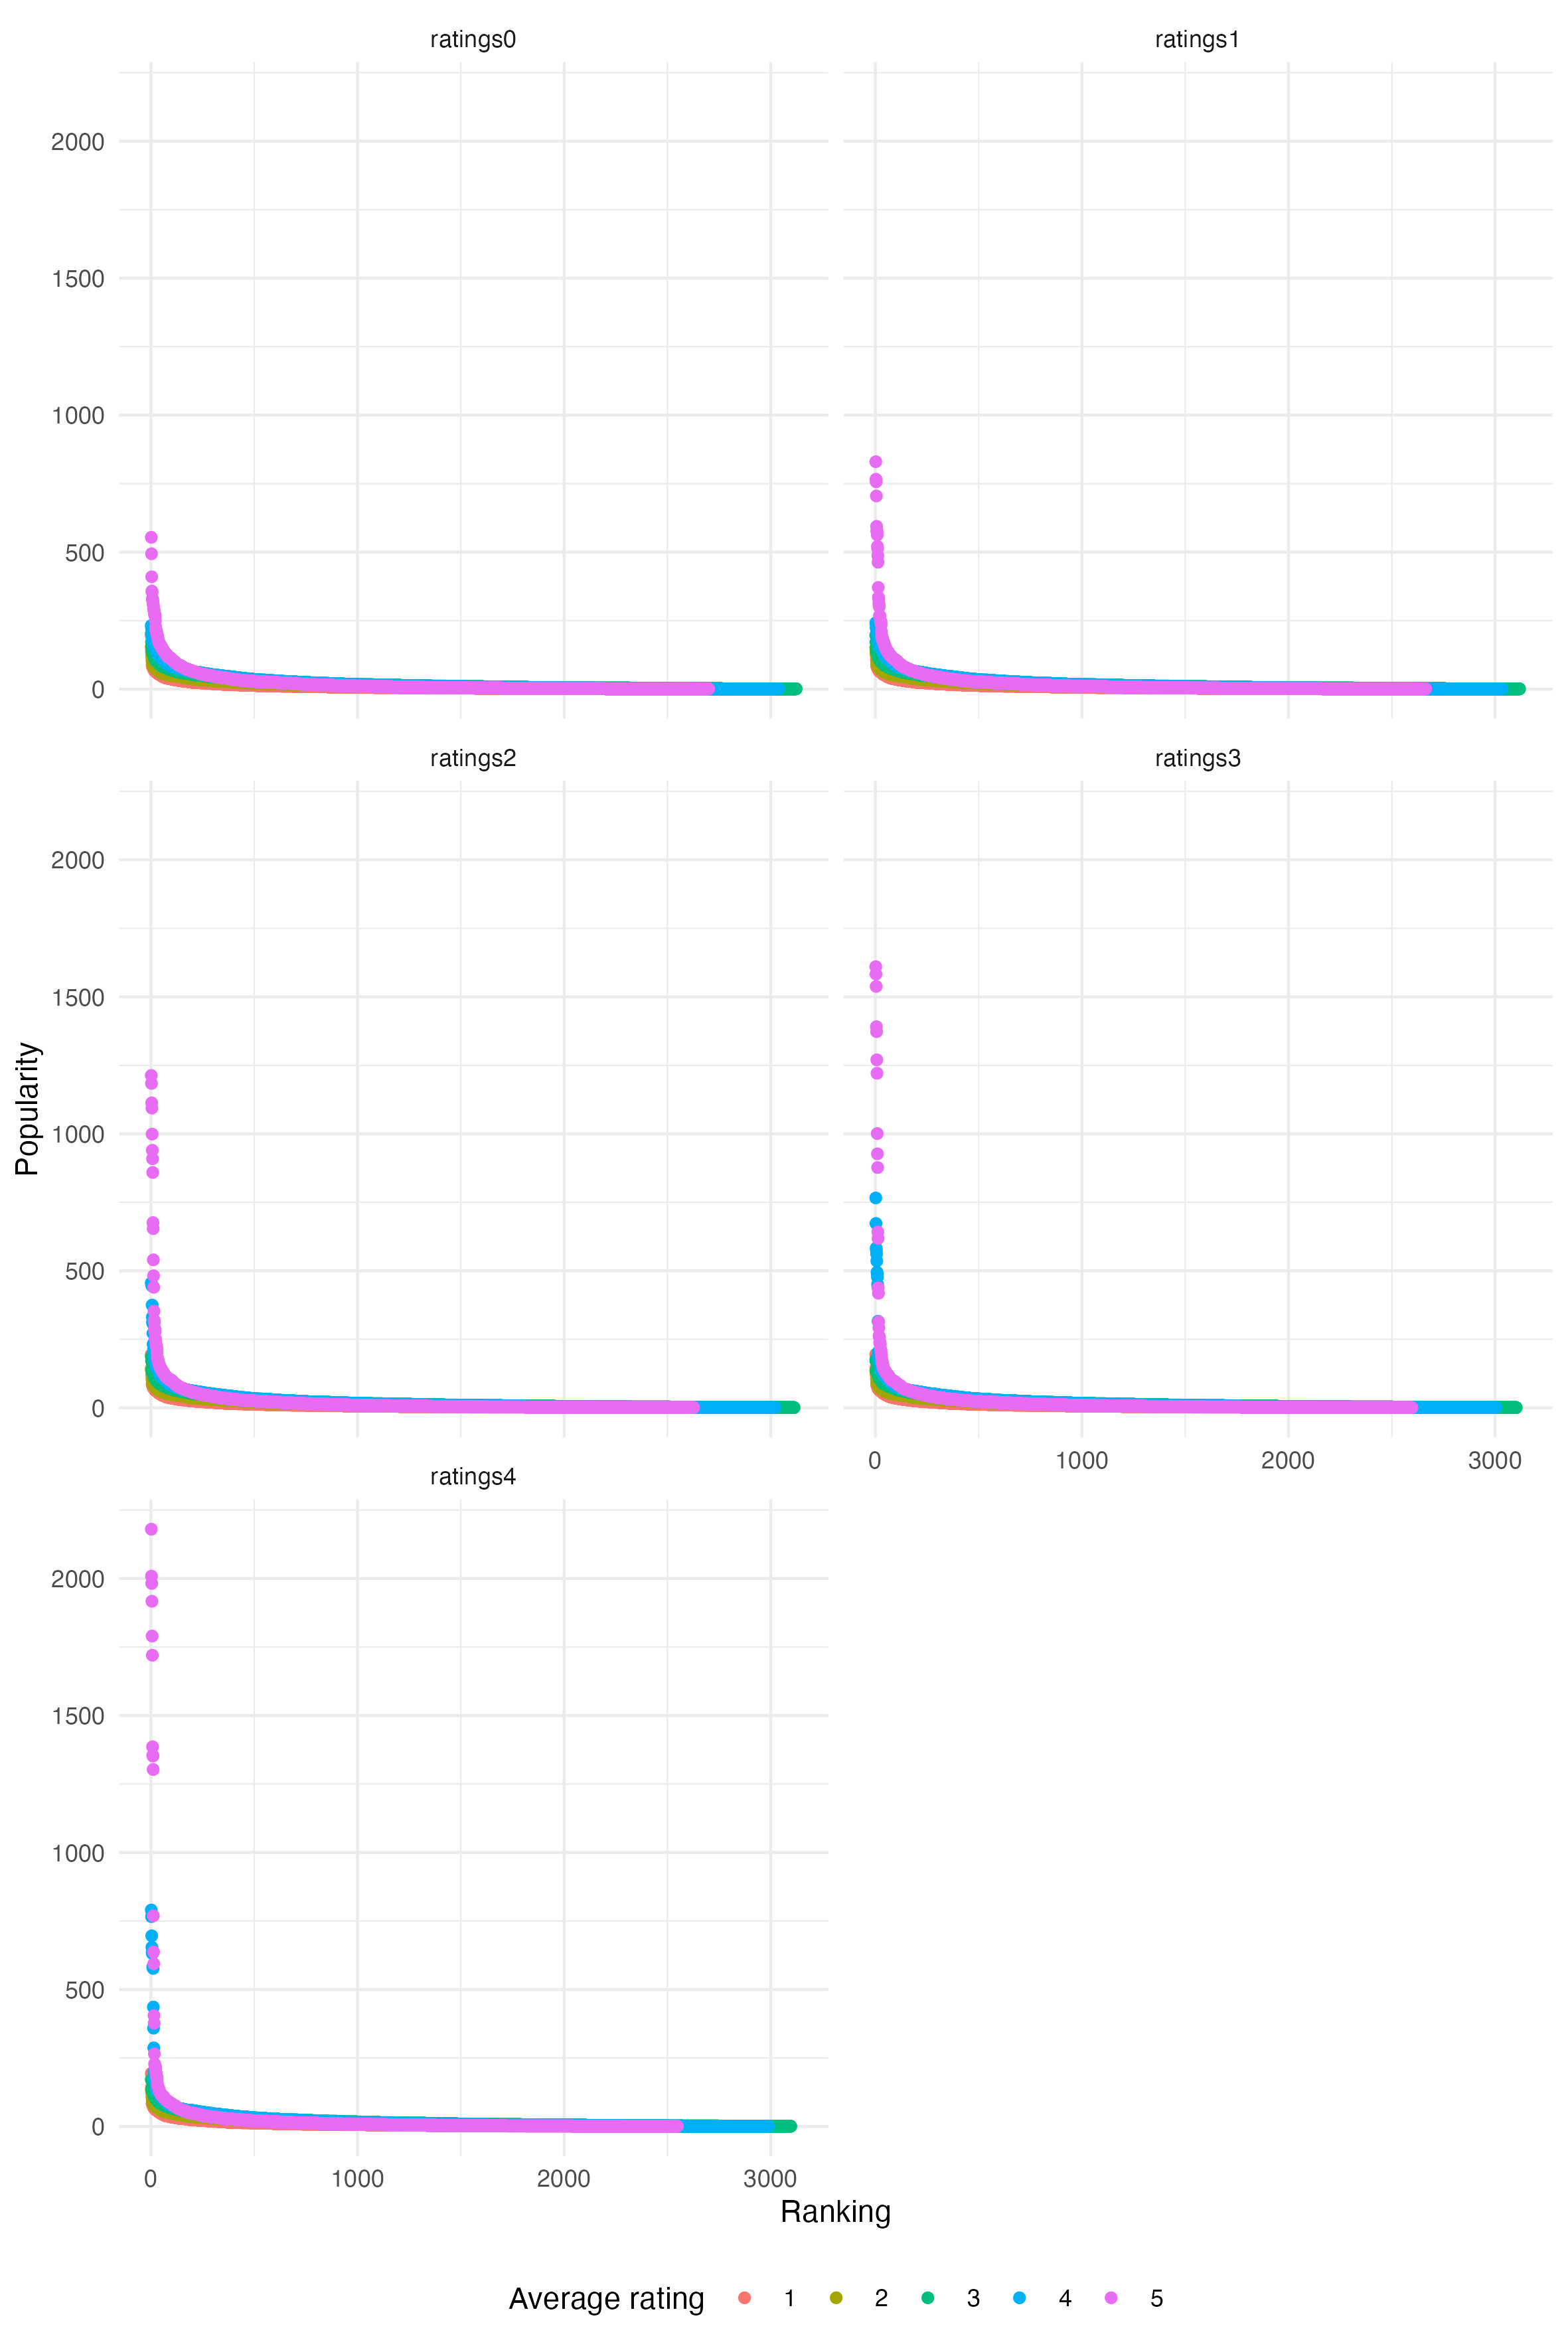
\includegraphics[width=\textwidth]{04_profile_grouped}
  \caption{Recommendation profile of every generation. Colors indicate average
  movie rating, which is a strong predictor of popularity over time.
  \label{fig:fig04_profile_grouped}}
\end{figure}

As explained before, we expected that movies which where already popular would
be recommended more times, but these plots indicate a powerful feedback loop.
Examining the data, we saw that the algorithm was consistently recommending
movies which the users had already watched and this process only became more
accentuated with each subsequent iteration. This is in line with recommendations
from large social networks like YouTube, which do recommend videos that were
already watched by the user.

Table~\ref{tab:tab04_top10_sum} contains the most recommended movies of every
generation of the experiment. Just as in Chapter~\ref{cap:static}, the number of
"recommendations" of generation 0 (i.e. the original dataset) is taken to be the
number of reviews each movie received. It is remarkable that the most
recommended movies in generation 4 were neither the most popular nor the highest
rated in generation 0. The full table (with movie names) can be seen in
Appendix~\ref{apx:pop}.

\begin{table}
\begin{tabular}{|r|r|r|r|r|r|}
  \hline
  & \multicolumn{5}{ c| }{Movie Recommendations} \\
  \hline
  ID & Generation 0 & Generation 1 & Generation 2 & Generation 3 & Generation 4\\
  \hline
  50 & 95 & 715 & 1292 & 1898 & 1888\\
  \hline
  260 & 160 & 140 & 772 & 750 & 738\\
  \hline
  318 & 115 & 705 & 1296 & 1908 & 2468\\
  \hline
  527 & 106 & 663 & 657 & 1256 & 1822\\
  \hline
  608 & 175 & 163 & 151 & 133 & 113\\
  \hline
  745 & 44 & 664 & 1252 & 1810 & 2436\\
  \hline
  858 & 103 & 669 & 1261 & 1861 & 2422\\
  \hline
  904 & 79 & 644 & 1252 & 1243 & 1814\\
  \hline
  922 & 36 & 601 & 1191 & 1786 & 2385\\
  \hline
  1148 & 47 & 629 & 1217 & 1808 & 2432\\
  \hline
  1198 & 99 & 520 & 500 & 1119 & 1718\\
  \hline
  1212 & 30 & 24 & 606 & 1172 & 1168\\
  \hline
  1580 & 174 & 156 & 134 & 113 & 98\\
  \hline
  2019 & 37 & 652 & 1276 & 1881 & 2496\\
  \hline
  2396 & 202 & 180 & 163 & 136 & 106\\
  \hline
  2628 & 165 & 149 & 135 & 115 & 97\\
  \hline
  2762 & 256 & 230 & 201 & 171 & 135\\
  \hline
  2858 & 198 & 170 & 148 & 134 & 111\\
  \hline
  2987 & 244 & 229 & 218 & 205 & 185\\
  \hline
  3176 & 197 & 186 & 172 & 159 & 136\\
  \hline
  3578 & 208 & 194 & 176 & 157 & 136\\
  \hline
  3793 & 210 & 204 & 189 & 179 & 158\\
  \hline
\end{tabular}
\caption{Every movie featured in the top 10 most recommended of at least one generation.}
\label{tab:tab04_top10_sum}
\end{table}

A good way to measure how diverse were the recommendations made by the algorithm
is to calculate the entropy \citep{borda_fundamentals_2011} of each set. This
metric is defined for a discrete random variable $X$, which can assume values
form the alphabet $\chi$, through the formula:

$$
H(X) = - \sum_{x \in \chi} p(x) \log p(x).
$$

In the extreme, if the same movie is recommended to every user, than the entropy
of the recommendations will tend to zero. In absolute terms, the entropy of
\verb|ratings0| was 7.42, and the entropy of \verb|ratings4| was 6.08 (18\%
lower). A comparison in relative terms is displayed in
Figure~\ref{fig:fig04_entropy}.

\begin{figure}
  \centering
  \begin{subfigure}{0.45\textwidth}
    \centering
    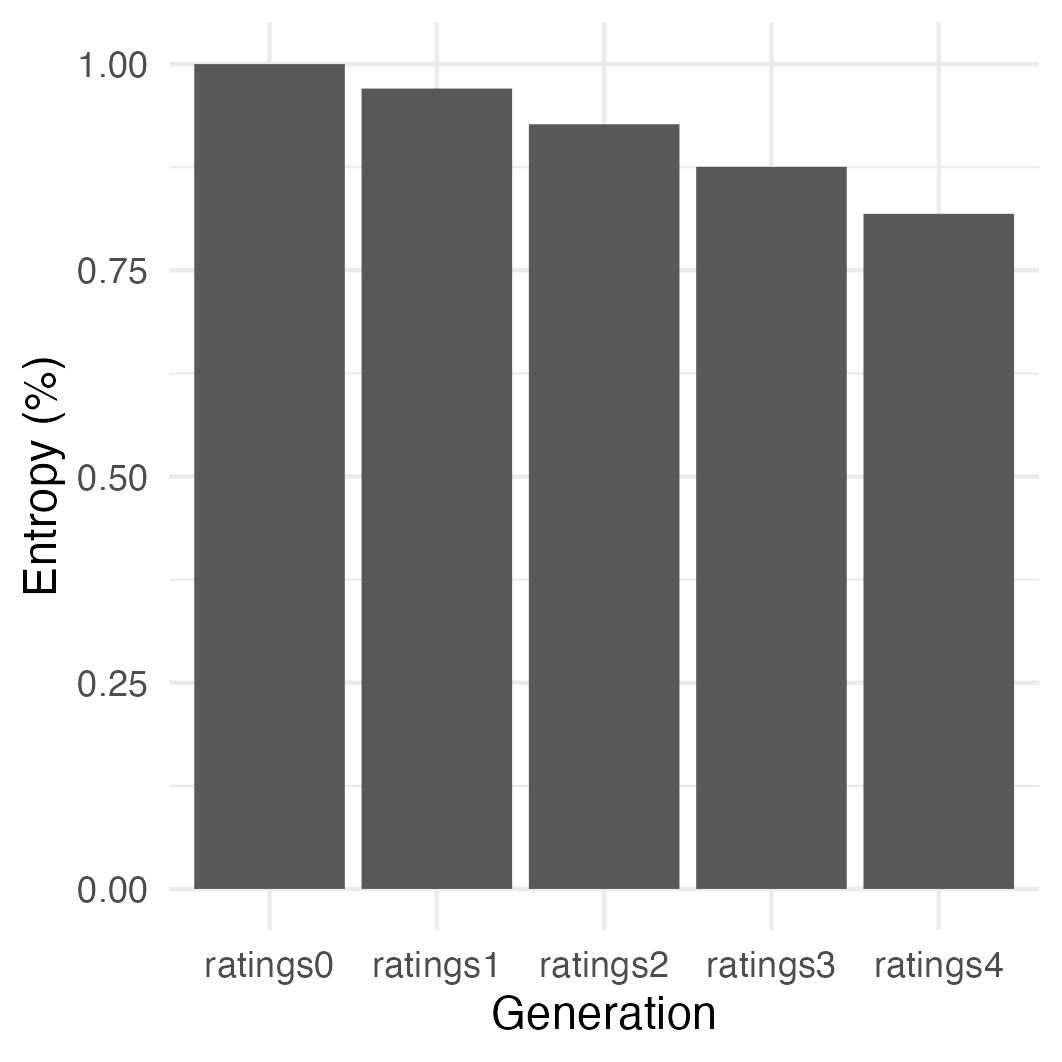
\includegraphics[width=\textwidth]{04_entropy}
  \end{subfigure}
  \caption{Recommendation entropy as a percentage of ratings0s entropy.
  \label{fig:fig04_entropy}}
\end{figure}

We can also observe this reduction of variety in an even more visual way. In
Figure~\ref{fig:fig04_popularity_time_both} we plotted movie popularity over
time; each line represents a movie and each step in the x-axis is a new
generation of the model. Figure~\ref{fig:fig04_popularity_time} makes it very
clear that only 13 movies rose in popularity over the four generations of the
recommendation system, becoming orders of magnitude more popular than the rest.
We also scaled the y-axis by taking the its log in
Figure~\ref{fig:fig04_log_popularity_time}, and we can see that, in fact, no
other movie rose in popularity besides the ones that stick out after
\verb|model2|.

It is also of note that the few movies that rise in popularity are not the most
popular ones from \verb|ratings0|, even though genre was the only metadata we
fed into the system. This uncovers a significant feature of the feedback loop we
observed in Figure~\ref{fig:fig04_profile_grouped}: the items that the algorithm
amplifies don't necessarily have to be the most mainstream, or in other words,
recommendation systems are able to boost content artificially.

\begin{figure}
  \centering
  \begin{subfigure}{0.45\textwidth}
    \centering
    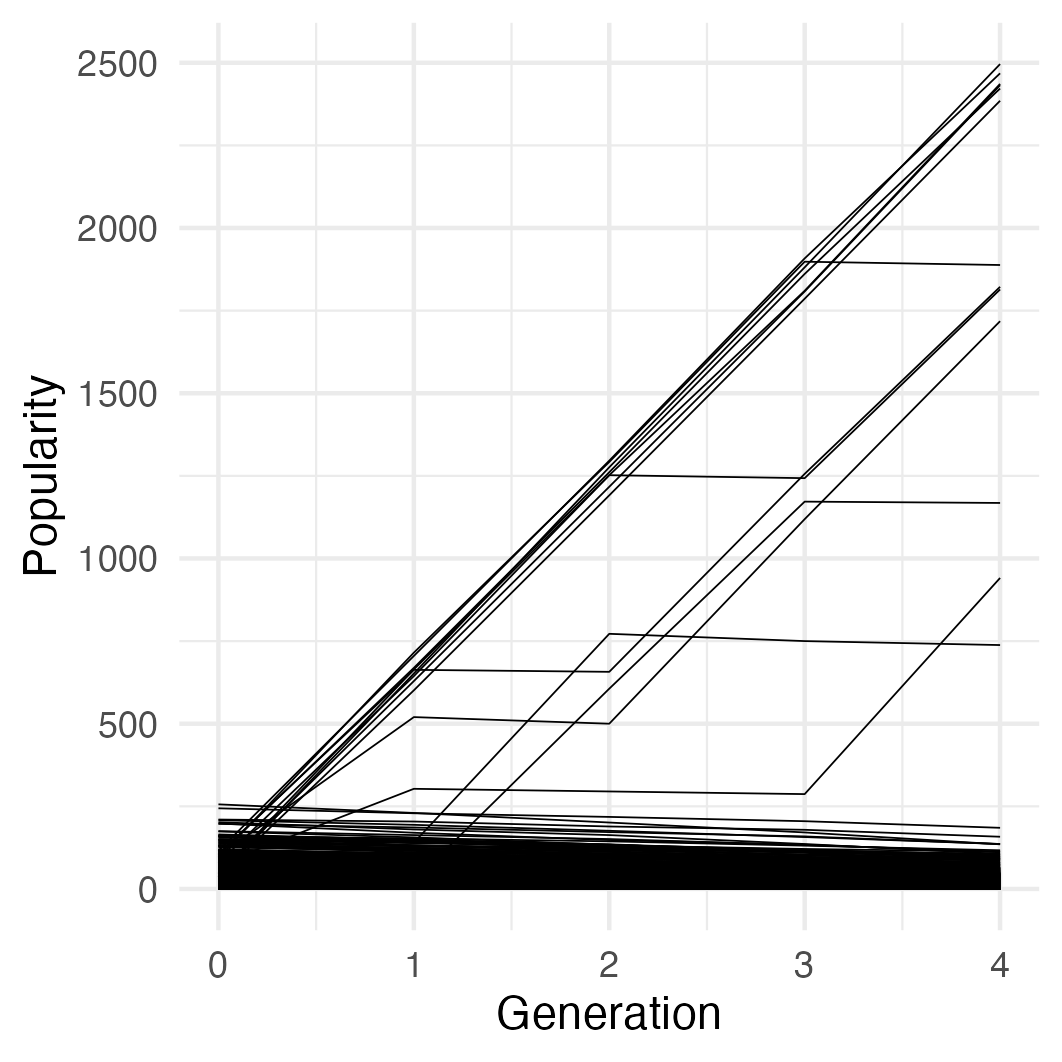
\includegraphics[width=\textwidth]{04_popularity_time}
    \caption{Movie popularity over time.\label{fig:fig04_popularity_time}}
  \end{subfigure}
  \begin{subfigure}{0.45\textwidth}
    \centering
    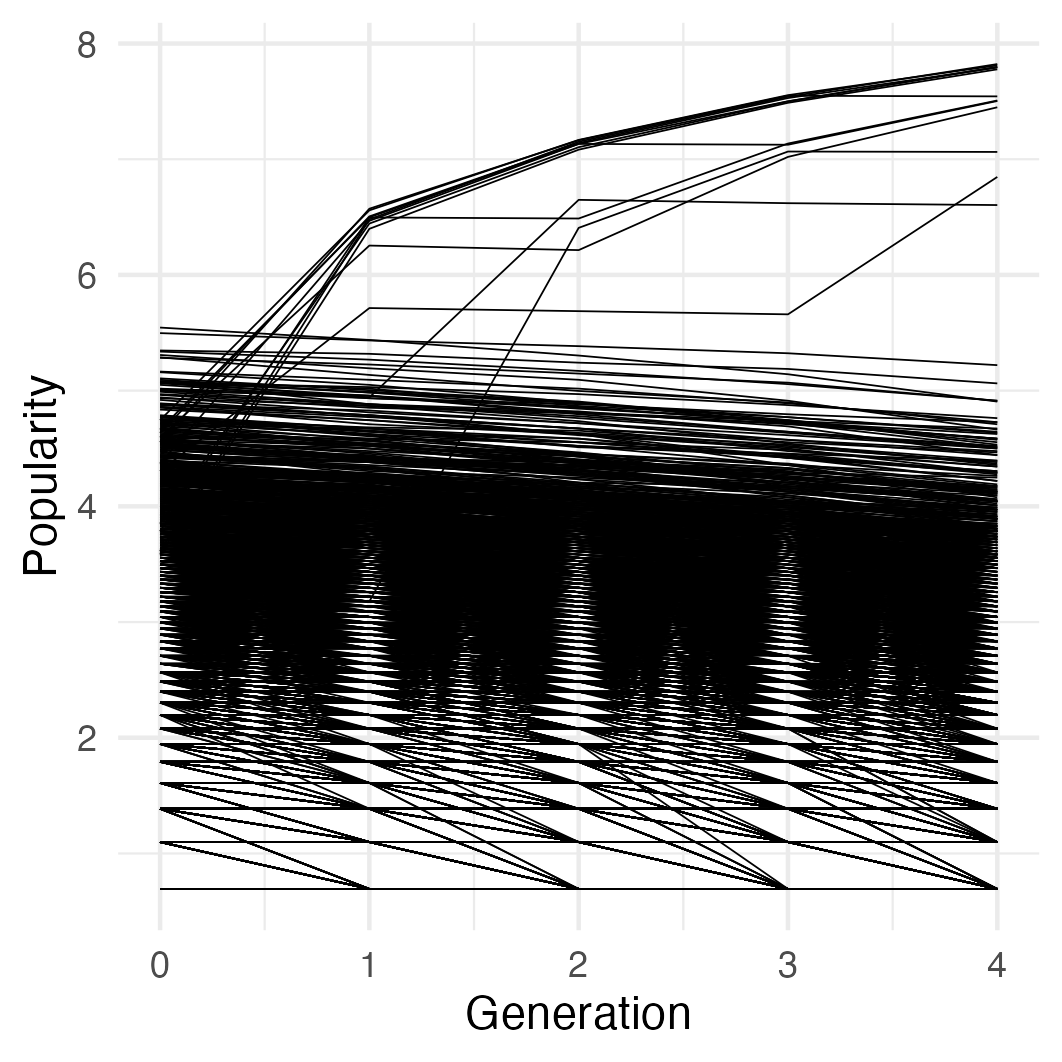
\includegraphics[width=\textwidth]{04_log_popularity_time}
    \caption{Movie log-popularity over time.\label{fig:fig04_log_popularity_time}}
  \end{subfigure}
  \caption{Popularity of every movie from ratings0 to ratings4.\label{fig:fig04_popularity_time_both}}
\end{figure}

\section{Modeling}
\label{sec:modeling04}

Deep learning models are extremely powerful and versatile; they are not,
however, very explainable \citep{roscher_explainable_2020}. Recommendation
algorithms are often described as black boxes because of the seemingly
inscrutable impact that different inputs have on the output. The term "neural
hallucination" \citep{raunak_curious_2021} has even been coined to explain the
process by which neural networks infer missing information form incomplete data.

Since we did identify a feedback loop in the recommendation system, our next
goal was to fit a regression model on the generated data. This could help
clarify how the algorithm had made it's recommendations; if we were able to
create a regression model that replicated the behavior of the system, then we
could make inferences about the algorithm based on the characteristics of said
model.

As is common in computational inference \citep{robert_james_2011}, our process
involved multiple rounds of modeling. We started with a very simple model and,
according to goodness-of-fit measurements, made it more and more complex in
order to achieve a better representation of the behavior of the recommendation
system. As we will see later, even after feeding all of the the available data
(and some extra metadata that the recommender algorithm didn't have access to),
our models were not able to capture such a degenerate distribution.

For every model described below, the response variable $Y$ is the number of
recommendations a movie received at a specific moment in time, while $\lambda$
is the average recommendation rate (conditioned to a movie's genre and rating)
at a specific moment in time.

\subsection{Poisson Regression}
\label{subsec:poisson04}

From the quasi-exponential decay observed in
Figure~\ref{fig:fig04_profile_grouped}, we hypothesized that the logarithm of
popularity was a function of the linear combination of genre, generation and
rating. Our first attempt was, therefore, a simple Poisson regression
\citep{allison_fixed-effects_2002}. For this kind of model, we fit a regression
of the form

$$
\log(\lambda_i) = \beta_0 + \beta_1 x_{i1} + \dots + \beta_k x_{ik},
$$

\noindent where $\lambda_i$ is the Poisson parameter, $x_{ik}$ is the regressor
variable, and $\beta_i$ is the regression coefficient. To implement the
regression, we used R's \verb|glm()| \citep{rcore_stats_2022} function with
popularity being modeled by the factor crossing of generation (i.e., the
iteration from 0 to 4), genre and average rating.

As the reader might be able to see, we used the genre variable in our regression
model even though we didn't feed it to the recommendation system. As explained
before, the algorithm only had access to the popularity and ratings of the
movies, but it is possible the there exists a latent effect of genre on the
other variables; since a machine learning system is much more flexible than a
regression model, we opted to explicitly feed the genre into the Poisson model
and all others that followed.

\verb|glm()| and all other regression functions return the coefficients of the
regression alongside their calculated significance. However, analyzing the
coefficients by themselves is only one part of the full picture.
\citet{atkinson_plots_1987} proposed the usage of simulated envelopes, alongside
coefficient significance, to assess global goodness-of-fit.

This method is such that, under the correct model, the plot for the observed
data is likely to fall within the envelope. The objective is not to provide a
region of acceptance, but some sort of guidance to what kind of shape to expect.

Obtaining the simulated envelope consists of fitting a model; extracting model
diagnostics and calculating sorted absolute values; simulating the desired
number of response variables using the same model matrix, error distribution and
fitted parameters; fitting the same model to each simulated response variable
and obtaining the same model diagnostics, again sorted absolute values; and
computing the desired percentiles (in this case, 2.5\% and 97.5\%) at each value
of the expected order statistic to form the envelope. In our case, the expected
order statistic was obtained through the following normal distribution:

$$
\Phi^{-1}(\frac{i+3/8}{n+1/4})
$$

For illustrative purposes, we will present the full output of the Poisson model
below. It is notable how many coefficients are considered highly significant,
meaning that, individually, they were able to capture the feedback loop
generated by the recommendation system.

\begin{verbatim}
Call:
glm(formula = pop ~ t * genre * rating, family = "poisson", data = features)

Deviance Residuals:
    Min       1Q   Median       3Q      Max
-33.145   -3.088   -1.222    1.260   93.001

Coefficients:
                            Estimate Std. Error z value Pr(>|z|)
(Intercept)                9.210e-02  9.514e-02   0.968 0.333031
t                         -6.844e-02  4.200e-02  -1.629 0.103208
genreAnimation            -2.276e+00  1.475e-01 -15.430  < 2e-16 ***
genrechildren's            1.489e-02  1.754e-01   0.085 0.932347
genreComedy               -1.904e-01  1.041e-01  -1.828 0.067539 .
genreCrime                -4.898e+00  1.858e-01 -26.364  < 2e-16 ***
genreDocumentary          -1.801e+00  4.491e-01  -4.010 6.07e-05 ***
genreDrama                -1.035e+00  1.140e-01  -9.086  < 2e-16 ***
genreFilm-Noir            -1.631e+01  5.403e-01 -30.185  < 2e-16 ***
genreHorror                3.012e-01  1.178e-01   2.556 0.010582 *
genreMusical              -2.784e+00  4.813e-01  -5.784 7.31e-09 ***
genreMystery              -4.849e+00  2.464e-01 -19.681  < 2e-16 ***
genreRomance              -1.476e+00  5.299e-01  -2.785 0.005347 **
genreSci-Fi                1.583e+00  1.898e-01   8.341  < 2e-16 ***
genreThriller              3.854e-01  1.791e-01   2.152 0.031394 *
genreWestern              -4.253e+00  5.017e-01  -8.476  < 2e-16 ***
rating                     8.877e-01  2.740e-02  32.395  < 2e-16 ***
t:genreAnimation          -3.139e+00  6.223e-02 -50.435  < 2e-16 ***
t:genrechildren's         -5.212e-04  7.760e-02  -0.007 0.994641
t:genreComedy             -2.235e-02  4.602e-02  -0.486 0.627215
t:genreCrime              -3.561e+00  8.570e-02 -41.557  < 2e-16 ***
t:genreDocumentary         2.463e-01  1.933e-01   1.274 0.202583
t:genreDrama              -1.845e+00  5.015e-02 -36.799  < 2e-16 ***
t:genreFilm-Noir          -5.419e+00  1.944e-01 -27.872  < 2e-16 ***
t:genreHorror              7.776e-03  5.217e-02   0.149 0.881511
t:genreMusical             1.190e-01  2.140e-01   0.556 0.578236
t:genreMystery            -3.676e+00  1.032e-01 -35.632  < 2e-16 ***
t:genreRomance            -8.909e-02  2.334e-01  -0.382 0.702658
t:genreSci-Fi             -2.251e+00  8.076e-02 -27.869  < 2e-16 ***
t:genreThriller            6.362e-02  7.894e-02   0.806 0.420240
t:genreWestern             5.290e-02  2.211e-01   0.239 0.810874
t:rating                  -1.584e-02  1.212e-02  -1.307 0.191193
genreAnimation:rating      7.049e-01  3.938e-02  17.900  < 2e-16 ***
genrechildren's:rating    -4.814e-02  5.303e-02  -0.908 0.364006
genreComedy:rating         1.711e-02  2.989e-02   0.572 0.567055
genreCrime:rating          1.261e+00  4.818e-02  26.161  < 2e-16 ***
genreDocumentary:rating    5.638e-02  1.160e-01   0.486 0.626776
genreDrama:rating          1.163e-01  3.199e-02   3.635 0.000278 ***
genreFilm-Noir:rating      3.865e+00  1.239e-01  31.197  < 2e-16 ***
genreHorror:rating        -1.456e-01  3.541e-02  -4.111 3.95e-05 ***
genreMusical:rating        6.395e-01  1.255e-01   5.095 3.50e-07 ***
genreMystery:rating        1.286e+00  6.114e-02  21.030  < 2e-16 ***
genreRomance:rating        3.492e-02  1.506e-01   0.232 0.816639
genreSci-Fi:rating        -5.037e-01  5.457e-02  -9.230  < 2e-16 ***
genreThriller:rating      -1.952e-01  5.094e-02  -3.833 0.000127 ***
genreWestern:rating        9.773e-01  1.309e-01   7.467 8.19e-14 ***
t:genreAnimation:rating    8.263e-01  1.631e-02  50.671  < 2e-16 ***
t:genrechildren's:rating  -1.370e-03  2.350e-02  -0.058 0.953503
t:genreComedy:rating       6.194e-03  1.323e-02   0.468 0.639610
t:genreCrime:rating        9.129e-01  2.163e-02  42.204  < 2e-16 ***
t:genreDocumentary:rating -5.843e-02  5.002e-02  -1.168 0.242813
t:genreDrama:rating        5.028e-01  1.399e-02  35.927  < 2e-16 ***
t:genreFilm-Noir:rating    1.279e+00  4.402e-02  29.061  < 2e-16 ***
t:genreHorror:rating      -6.526e-03  1.573e-02  -0.415 0.678237
t:genreMusical:rating     -3.530e-02  5.588e-02  -0.632 0.527603
t:genreMystery:rating      9.553e-01  2.495e-02  38.291  < 2e-16 ***
t:genreRomance:rating      3.023e-02  6.624e-02   0.456 0.648140
t:genreSci-Fi:rating       6.707e-01  2.195e-02  30.551  < 2e-16 ***
t:genreThriller:rating    -1.870e-02  2.252e-02  -0.830 0.406351
t:genreWestern:rating     -1.209e-02  5.768e-02  -0.210 0.834031
---
Signif. codes:  0 '***' 0.001 '**' 0.01 '*' 0.05 '.' 0.1 ' ' 1

(Dispersion parameter for poisson family taken to be 1)

    Null deviance: 562028  on 13559  degrees of freedom
Residual deviance: 268737  on 13500  degrees of freedom
AIC: 318813

Number of Fisher Scoring iterations: 6
\end{verbatim}

When we look at the simulated envelope of this regression, however, it is plain
to see that the model does not conform to the delimited region and, therefore,
isn't able to properly capture the variability of the data. The plot generated
with the \verb|hnp| \citep{moral_half-normal_2017} R package can be seen in
Figure~\ref{fig:fig04_residual_poisson}.

\begin{figure}
  \centering
  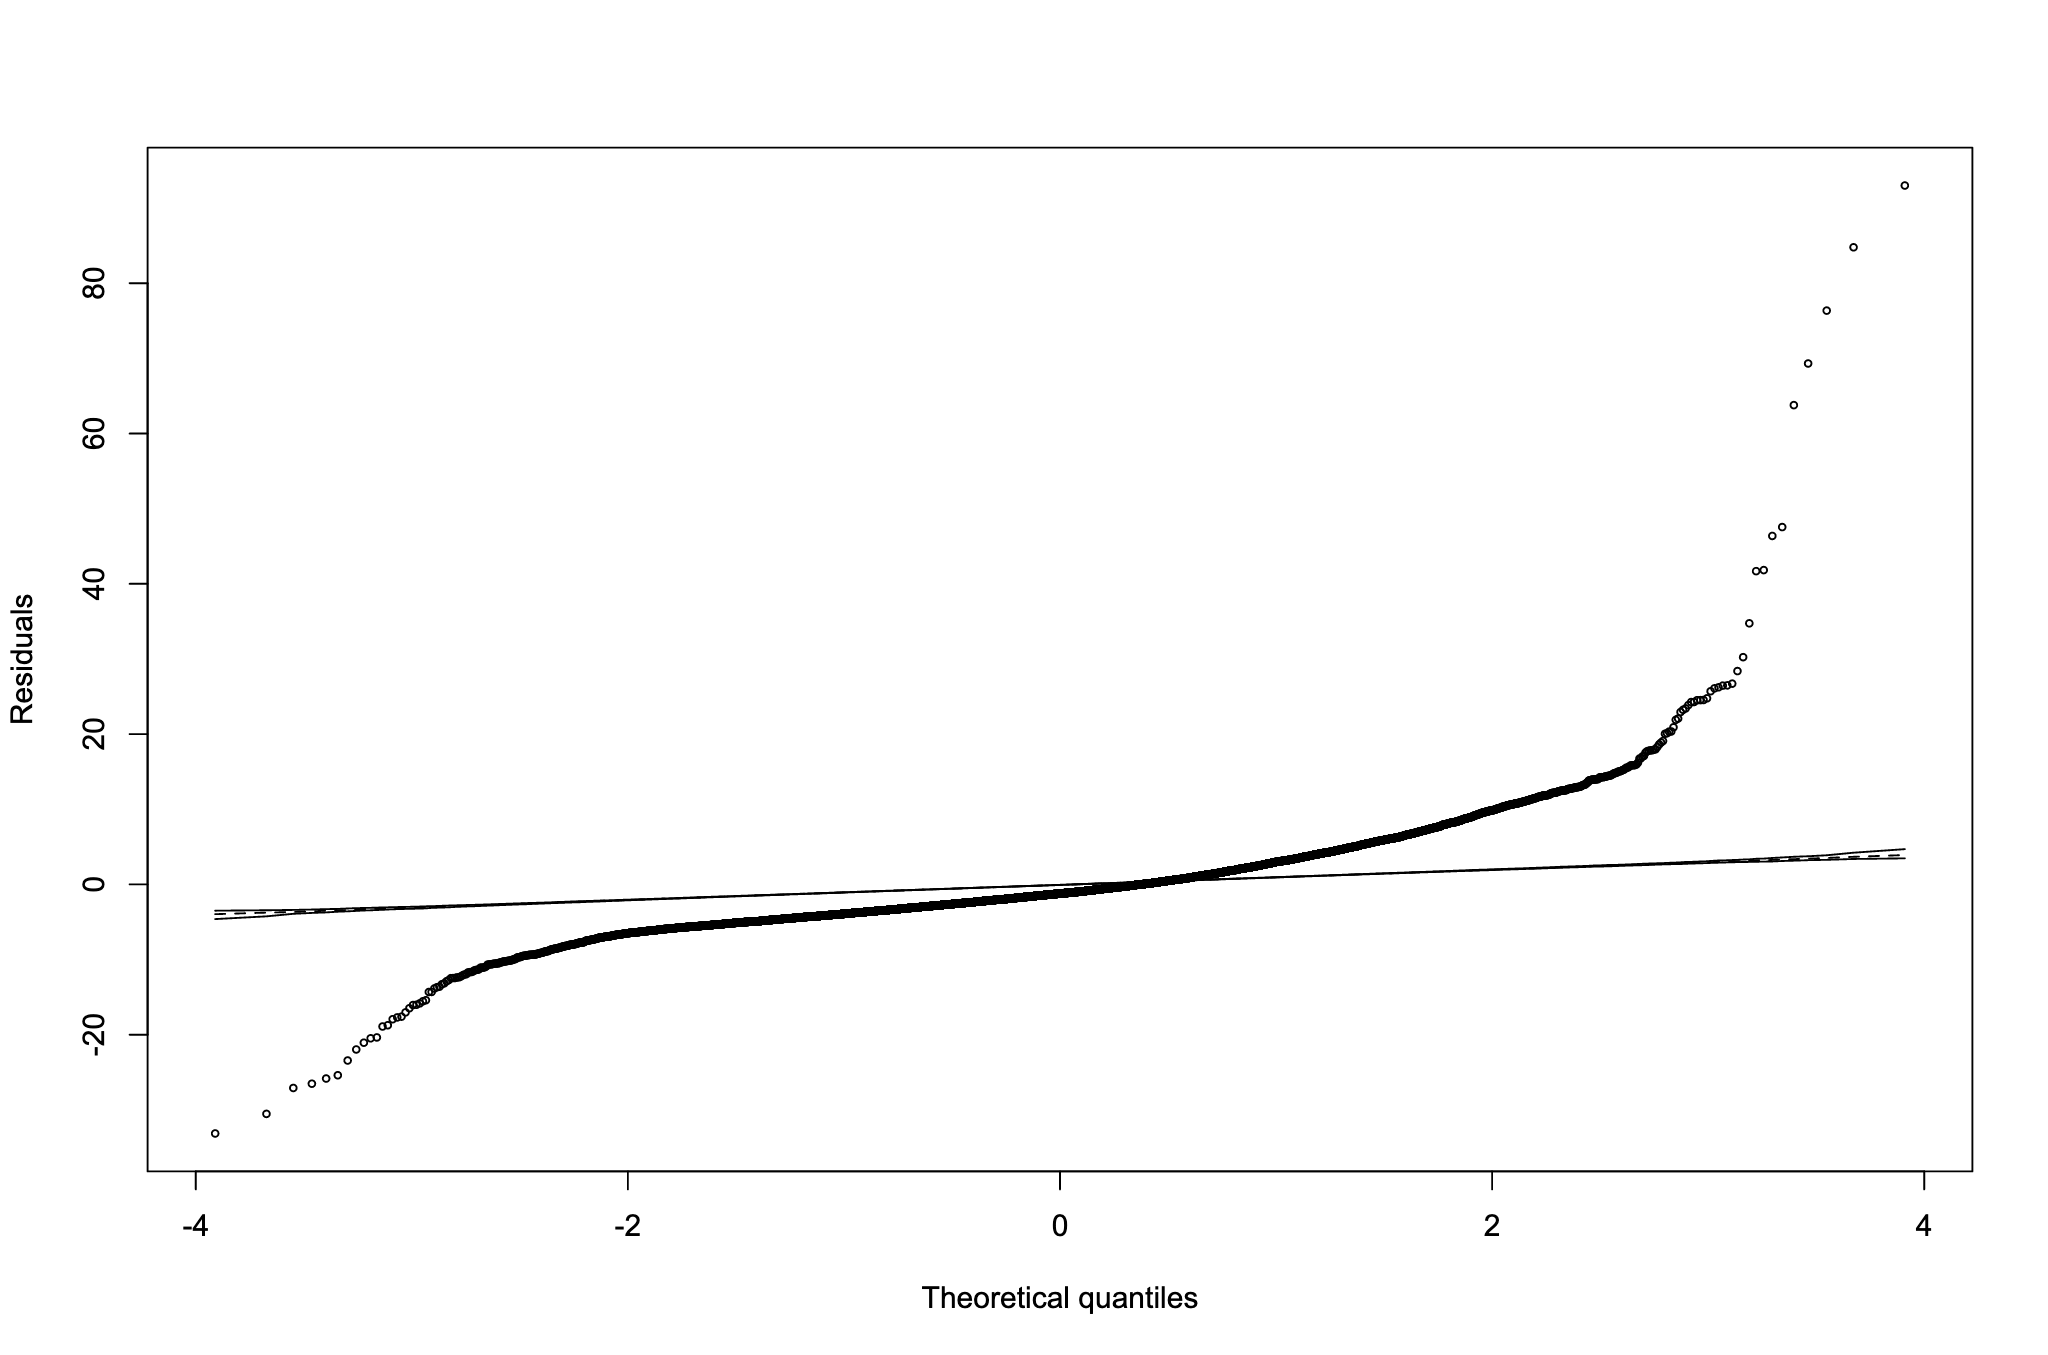
\includegraphics[width=\textwidth]{04_residual_poisson}
  \caption{Residual analysis via simulated envelope for the Poisson regression.\label{fig:fig04_residual_poisson}}
\end{figure}

\subsection{Negative Binomial Regression}
\label{subsec:negbin04}

Our next attempt involved a generalization of the previous regression. In a
Poisson model, both mean and variance are assumed to be the same; this could be
limiting our previous attempt, since it cannot capture overdispersed data. The
negative binomial distribution is a generalization of the Poisson distribution
\citep{allison_fixed-effects_2002} that is able to better model data under these
new assumptions. For this kind of model, we fit a regression of the form

$$
\log(\lambda_i) = \beta_0 + \beta_1 x_{i1} + \dots + \beta_k x_{ik},
$$

\noindent where $\lambda_i$ depends on covariates, as does $x_{ik}$. More
concretely, we used MASS's \citep{venables_modern_2002} \verb|glm.nb()| function
with the same formula as last time.

In this instance, the significancy of the coefficients of the regression
(omitted) was even higher than of the Poisson model. However, upon calculating
the simulated envelope, as seen in Figure~\ref{fig:fig04_residual_nb}, it became
clear that  this model, while better than the last, still was not adequately
capturing the data's variability.

\begin{figure}
  \centering
  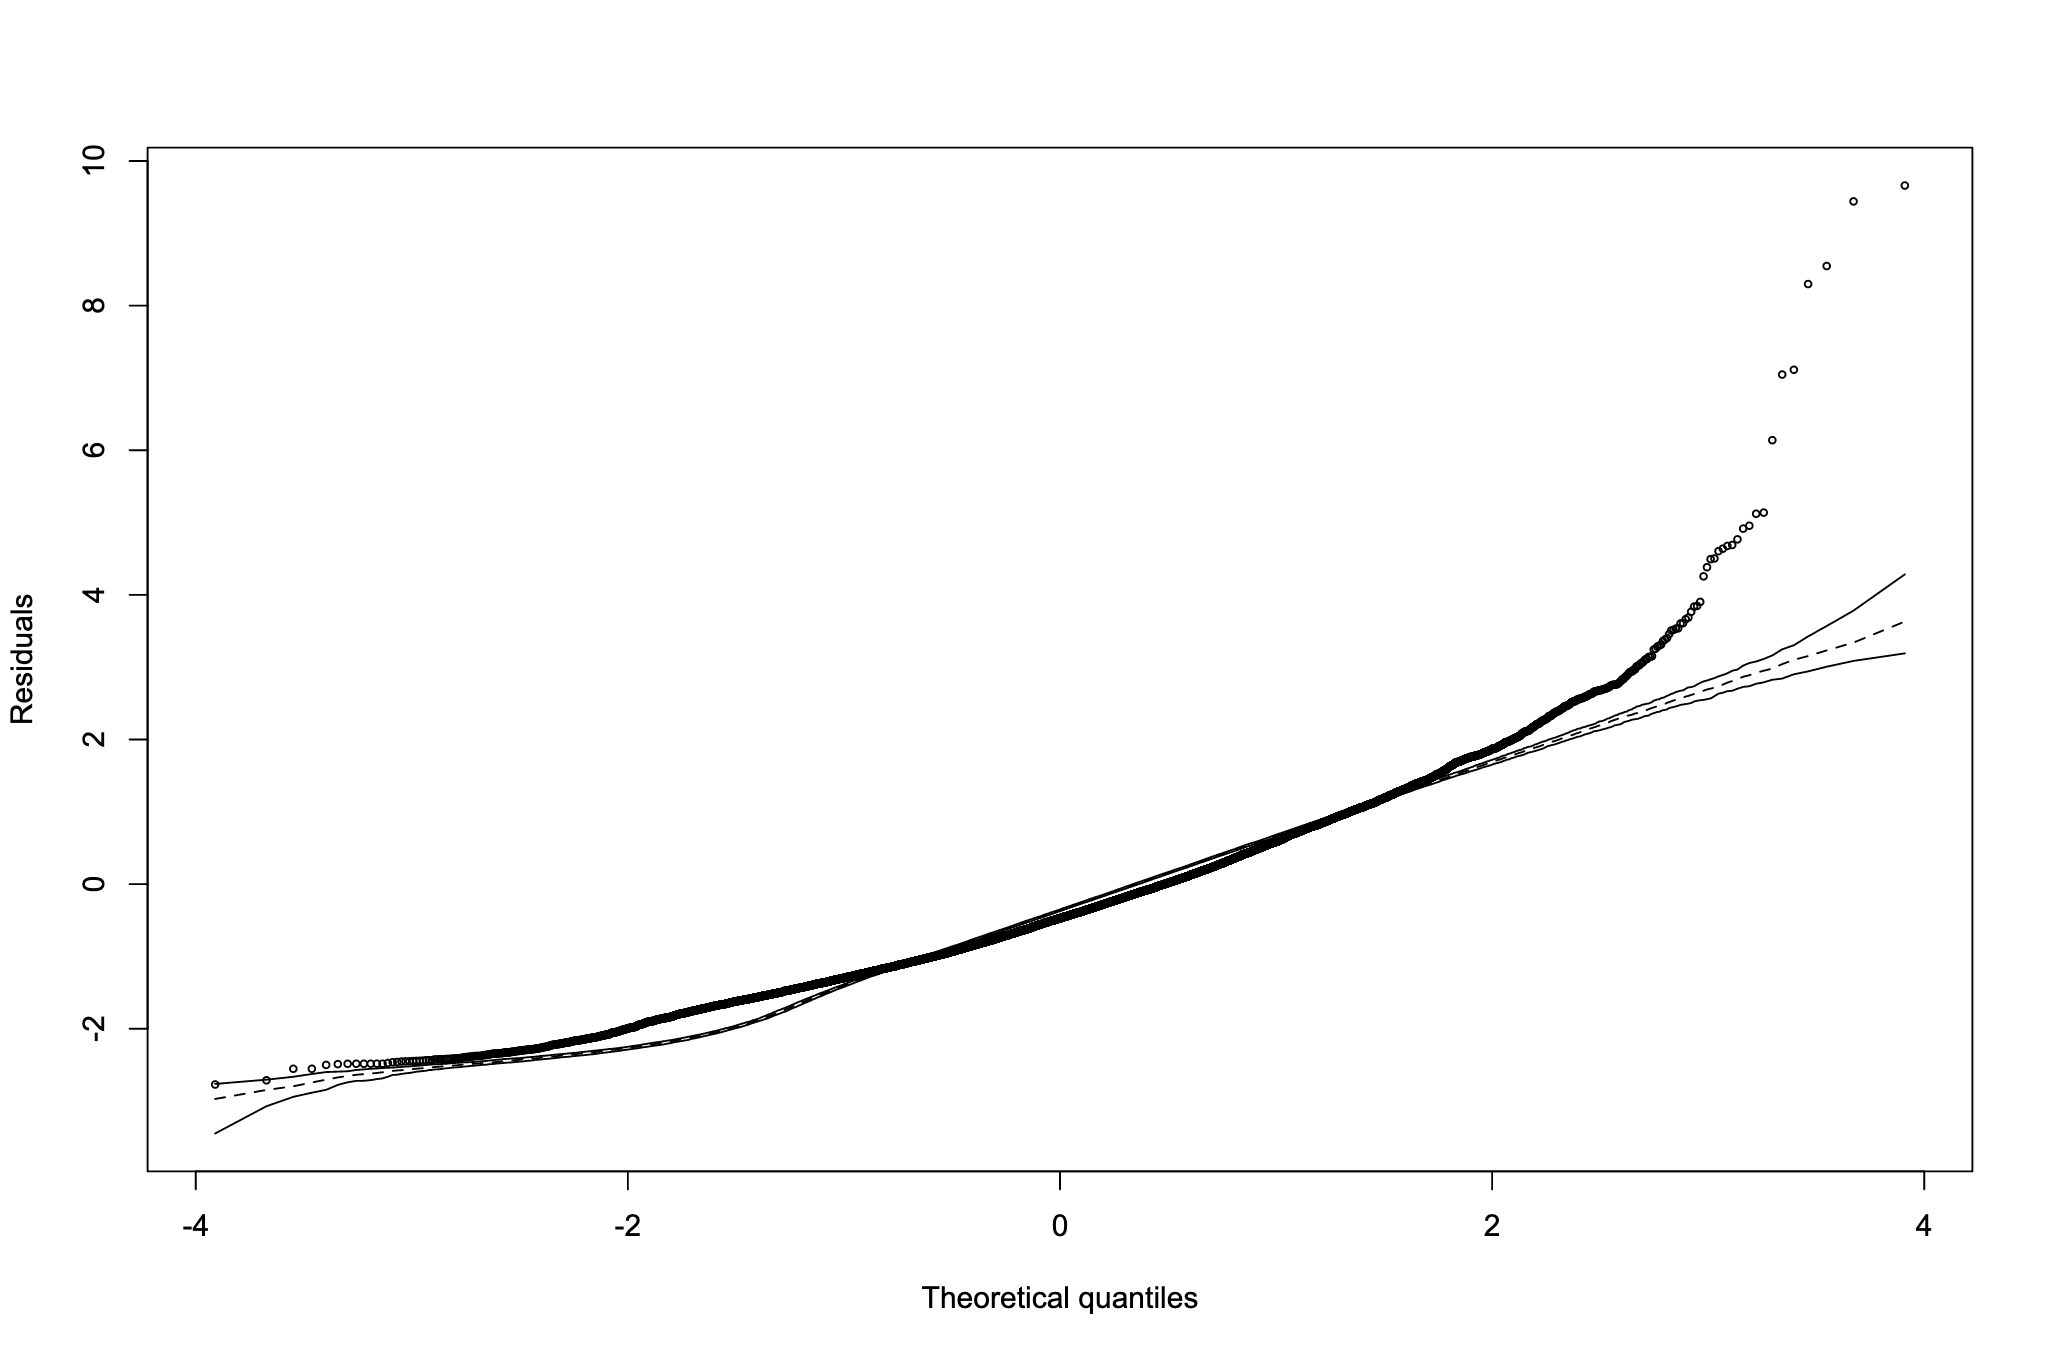
\includegraphics[width=\textwidth]{04_residual_nb}
  \caption{Residual analysis via simulated envelope for the negative binomial regression.\label{fig:fig04_residual_nb}}
\end{figure}

\subsection{Mixed-effects Poisson Regression}
\label{subsec:mmpoisson04}

Since both previous models failed to accurately capture the algorithm's
recommendation profile, we moved on to mixed-effects models given their
usefulness in longitudinal studies \citep{gomes_should_2022}. With this kind of
model we would be able to vary the coefficients from movie to movie, allowing
some movies to have steeper recommendation profiles than others.

The Poisson mixed-effects model can be generalized \citep{noauthor_applied_2023}
from the standard model by adding normally distributed random-effects to the
usual fixed-effects already described:

$$
\log(\lambda_i) = \delta + \beta_0 + \beta_1 x_{i1} + \dots + \beta_k x_{ik},
$$

\noindent where $\delta \sim \mathcal{N}(0,\psi)$ allows us to better model
longitudinal observations within the same individual (which are not independent
of each other) and serially correlated errors. In our regression, we added
mixed-effects to the \verb|movie_id| variable using the \verb|glmmTMB|
\citep{brooks_glmmtmb_2017} R package.

As with our previous regressions, we evaluate the fit of the model not only
through the significancy of the coefficients (which were on par with the other
models), but also through the simulated envelope. Since we used a different R
package to run the mixed-effects models, we also had to resort to another
simulation package: \verb|DHARMa| \citep{florian_dharma_2022}; this means that
the new plots in Figure~\ref{fig:fig04_residual_mmpois} follow a different
aesthetic convention and displays more information by default.

\begin{figure}
  \centering
  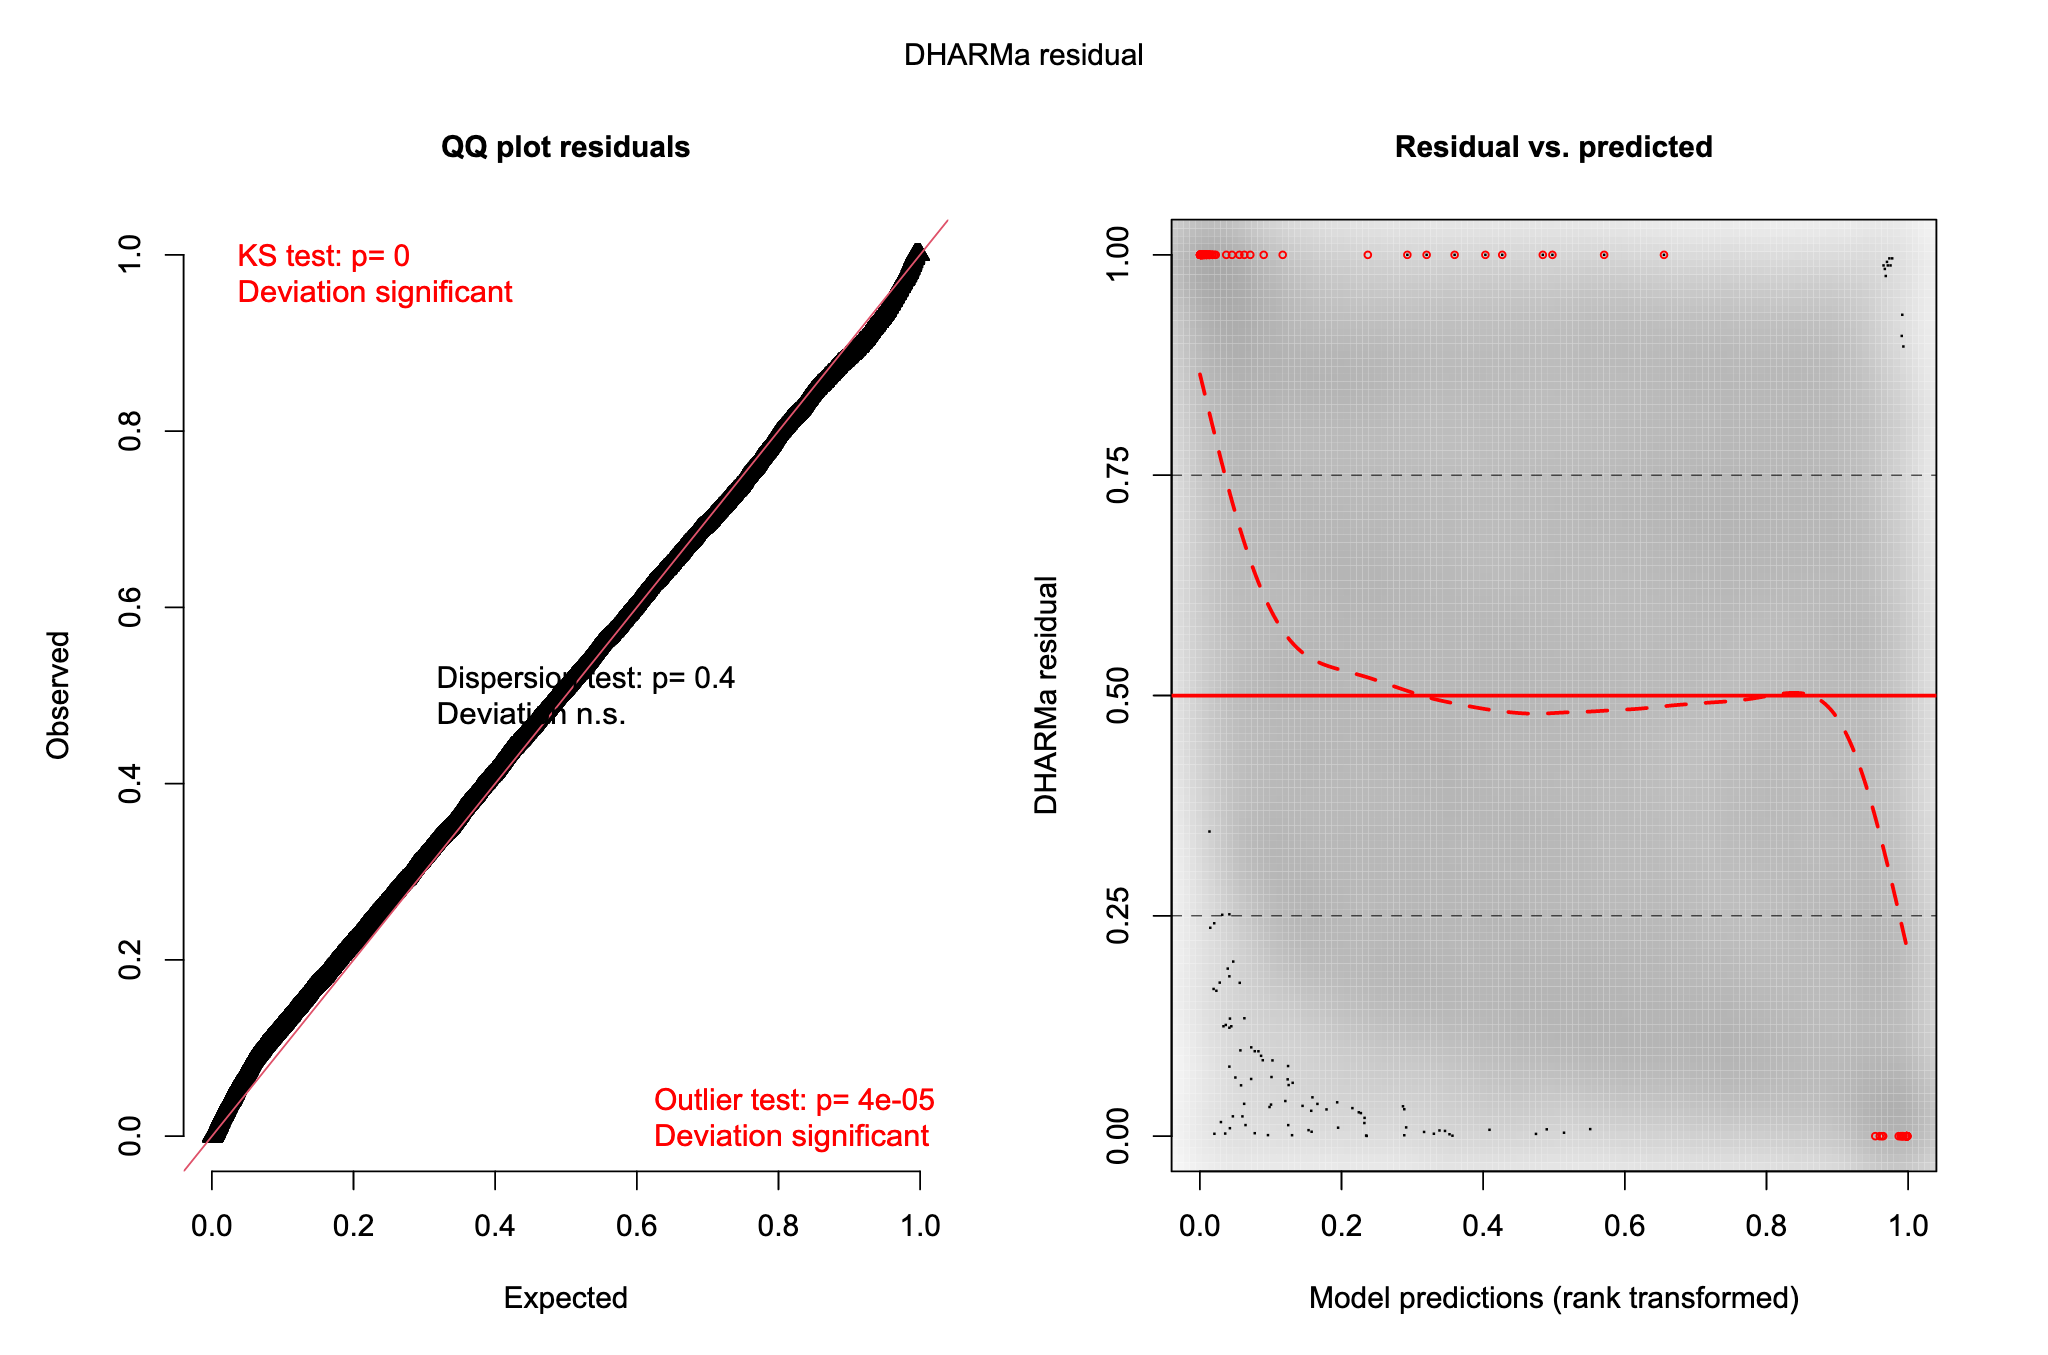
\includegraphics[width=\textwidth]{04_residual_mmpois}
  \caption{Residual analysis via simulated envelope for the mixed-effects Poisson regression.\label{fig:fig04_residual_mmpois}}
\end{figure}

Note how the fit is much better than the fixed-effects models, but the outliers
on the left and right sides of the distribution are still present as attested by
the outlier deviation test.

\subsection{Mixed-effects Negative Binomial Regression}
\label{subsec:mmnegbin04}

Our last attempt at capturing the recommendation profile of the recommender
system involved using a negative binomial mixed-model regression in order to
help with the overdispersion seen above. Similar to the Poisson mixed-effects
model, this regression also extends the default formula of its fixed-effects
counterpart:

$$
\log(\lambda_i) = \delta + \beta_0 + \beta_1 x_{i1} + \dots + \beta_k x_{ik}.
$$

In the table below, the reader can see the full summary of the negative binomial
mixed model. Figure~\ref{fig:fig04_residual_mmnb2} showcases the simulated
envelope for the same model.

\begin{verbatim}
  Family: nbinom2  ( log )
Formula:          pop ~ t * genre * rating + (1 | movie_id)
Data: features

    AIC      BIC   logLik deviance df.resid
83863.8  84370.3 -41865.9  83731.8    15844

Random effects:

Conditional model:
Groups   Name        Variance Std.Dev.
movie_id (Intercept) 1.364    1.168
Number of obs: 15910, groups:  movie_id, 3182

Dispersion parameter for nbinom2 family ():   49

Conditional model:
                            Estimate Std. Error z value Pr(>|z|)
(Intercept)                -0.108714   0.272464  -0.399 0.689891
t                          -0.210272   0.021153  -9.941  < 2e-16 ***
genreAdventure              0.112129   0.574197   0.195 0.845174
genreAnimation             -2.286362   0.773873  -2.954 0.003132 **
genrechildren's             0.855196   0.755919   1.131 0.257915
genreComedy                -0.108159   0.352431  -0.307 0.758925
genreCrime                 -3.590470   0.850227  -4.223 2.41e-05 ***
genreDocumentary           -1.659325   1.508329  -1.100 0.271285
genreDrama                 -1.219969   0.409312  -2.981 0.002877 **
genreFilm-Noir            -16.633103   2.371128  -7.015 2.30e-12 ***
genreHorror                 0.512807   0.443025   1.158 0.247062
genreMusical               -4.259252   2.088483  -2.039 0.041410 *
genreMystery               -4.646920   1.461852  -3.179 0.001479 **
genreRomance               -2.118789   1.856289  -1.141 0.253699
genreSci-Fi                 0.363380   1.044431   0.348 0.727899
genreThriller               1.382908   0.855392   1.617 0.105944
genreWestern               -3.766758   2.108848  -1.786 0.074072 .
rating                      0.957533   0.085468  11.203  < 2e-16 ***
t:genreAdventure            0.161327   0.053403   3.021 0.002520 **
t:genreAnimation           -0.392012   0.067698  -5.791 7.01e-09 ***
t:genrechildren's           0.116028   0.066946   1.733 0.083068 .
t:genreComedy               0.119502   0.030504   3.918 8.94e-05 ***
t:genreCrime               -0.146821   0.085503  -1.717 0.085952 .
t:genreDocumentary          0.329357   0.195776   1.682 0.092507 .
t:genreDrama                0.005393   0.038739   0.139 0.889287
t:genreFilm-Noir           -0.730742   0.227275  -3.215 0.001303 **
t:genreHorror               0.148203   0.041813   3.544 0.000393 ***
t:genreMusical              0.265118   0.243060   1.091 0.275383
t:genreMystery             -1.150785   0.123034  -9.353  < 2e-16 ***
t:genreRomance              0.064921   0.227735   0.285 0.775590
t:genreSci-Fi              -0.311108   0.079779  -3.900 9.63e-05 ***
t:genreThriller             0.134758   0.077077   1.748 0.080403 .
t:genreWestern              0.184582   0.216581   0.852 0.394073
t:rating                    0.029594   0.006273   4.717 2.39e-06 ***
genreAdventure:rating      -0.209253   0.179840  -1.164 0.244606
genreAnimation:rating       0.594327   0.226301   2.626 0.008633 **
genrechildren's:rating     -0.473591   0.247951  -1.910 0.056131 .
genreComedy:rating         -0.194909   0.109223  -1.785 0.074341 .
genreCrime:rating           0.736375   0.243050   3.030 0.002448 **
genreDocumentary:rating    -0.113489   0.399299  -0.284 0.776242
genreDrama:rating          -0.031020   0.120957  -0.256 0.797601
genreFilm-Noir:rating       3.958891   0.595316   6.650 2.93e-11 ***
genreHorror:rating         -0.422452   0.151685  -2.785 0.005352 **
genreMusical:rating         0.944897   0.569196   1.660 0.096903 .
genreMystery:rating         1.092607   0.409047   2.671 0.007560 **
genreRomance:rating         0.013712   0.548422   0.025 0.980053
genreSci-Fi:rating         -0.423339   0.324094  -1.306 0.191477
genreThriller:rating       -0.729129   0.256016  -2.848 0.004400 **
genreWestern:rating         0.725673   0.578412   1.255 0.209625
t:genreAdventure:rating    -0.053250   0.015828  -3.364 0.000768 ***
t:genreAnimation:rating     0.110189   0.018603   5.923 3.16e-09 ***
t:genrechildren's:rating   -0.039499   0.020922  -1.888 0.059031 .
t:genreComedy:rating       -0.039790   0.008913  -4.464 8.04e-06 ***
t:genreCrime:rating         0.038460   0.022654   1.698 0.089557 .
t:genreDocumentary:rating  -0.088874   0.050610  -1.756 0.079076 .
t:genreDrama:rating        -0.006800   0.010754  -0.632 0.527202
t:genreFilm-Noir:rating     0.183567   0.054187   3.388 0.000705 ***
t:genreHorror:rating       -0.052874   0.013574  -3.895 9.81e-05 ***
t:genreMusical:rating      -0.082105   0.063538  -1.292 0.196285
t:genreMystery:rating       0.335177   0.032553  10.296  < 2e-16 ***
t:genreRomance:rating      -0.018634   0.064877  -0.287 0.773939
t:genreSci-Fi:rating        0.108210   0.023442   4.616 3.91e-06 ***
t:genreThriller:rating     -0.044310   0.022584  -1.962 0.049758 *
t:genreWestern:rating      -0.055461   0.056878  -0.975 0.329521
---
Signif. codes:  0 '***' 0.001 '**' 0.01 '*' 0.05 '.' 0.1 ' ' 1
\end{verbatim}

\begin{figure}
  \centering
  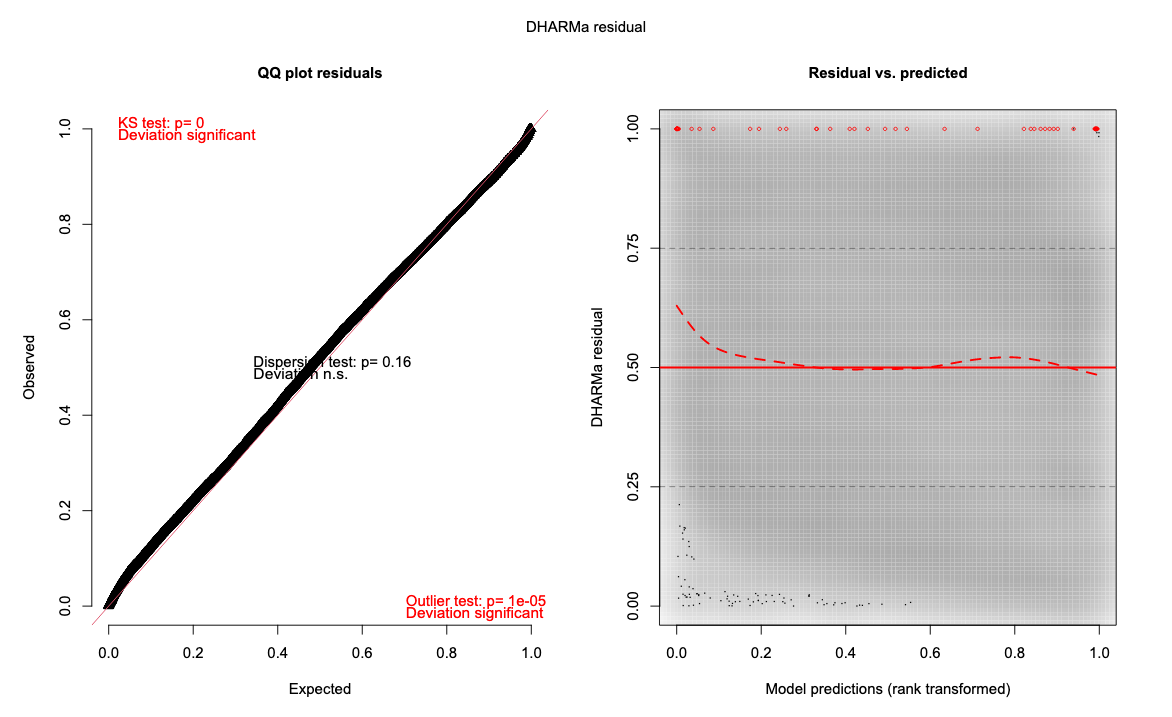
\includegraphics[width=\textwidth]{04_residual_mmnb2}
  \caption{Residual analysis via simulated envelope for the mixed-effects negative binomial regression.\label{fig:fig04_residual_mmnb2}}
\end{figure}

In comparison to the Poisson mixed model, the negative binomial mixed model is
2.5 times less dispersed and the outlier deviation is 4 times lower. Still, this
was not enough to capture accurately the recommendation profile of our system
for the more popular movies (left tail of the rightmost plot).

At this point, it is safe to assume that this distribution tends towards
degeneracy, meaning it approaches a situation
\citep{weisstein_degenerate_nodate} where only one movie is recommended every
single time and all others are never recommended.
